\documentclass[tikz,border=3pt]{standalone}
\usepackage[utf8]{inputenc}
\usepackage[T1]{fontenc}
\usepackage{lmodern}
\renewcommand{\familydefault}{\sfdefault}
\usepackage{sansmath}\sansmath
\usepackage{chemfig}
\usepackage{pgfplots}\pgfplotsset{compat=1.18,/pgf/number format/use comma,/pgf/number format/1000 sep={.}}
\usetikzlibrary{arrows.meta,calc,positioning,decorations.pathmorphing,patterns}
% paleta del sitio
\definecolor{nar}{HTML}{E8680C}\definecolor{narc}{HTML}{FFB35C}\definecolor{hielo}{HTML}{FFF3E8}
\definecolor{tinta}{HTML}{1D1D1F}\definecolor{gris}{HTML}{6E6E73}\definecolor{lila}{HTML}{7C5CF0}
\definecolor{azul}{HTML}{2F6FD6}\definecolor{menta}{HTML}{17A673}\definecolor{coral}{HTML}{E8342A}
\begin{document}
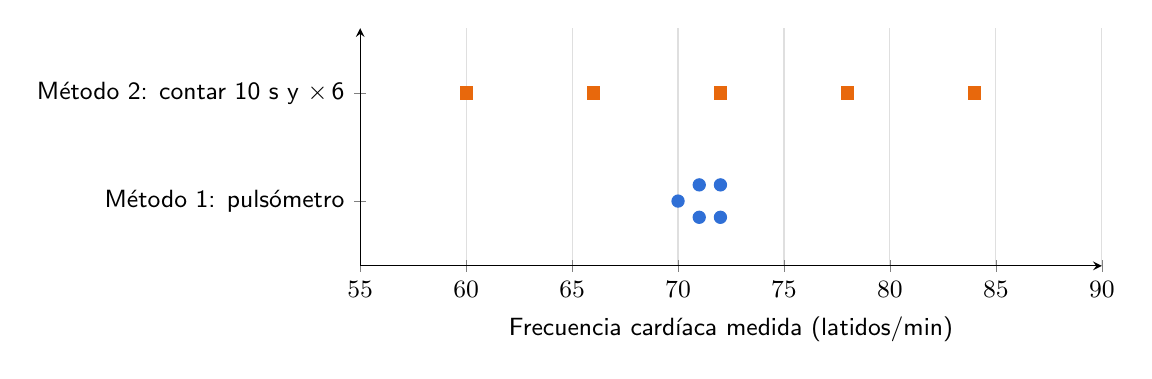
\begin{tikzpicture}[font=\small]
\begin{axis}[width=11cm,height=4.6cm,axis lines=left,xmin=55,xmax=90,ymin=0.4,ymax=2.6,xtick={55,60,...,90},
  ytick={1,2},yticklabels={{Método 1: pulsómetro},{Método 2: contar 10 s y $\times$\,6}},
  xmajorgrids,grid style={gray!25},xlabel={Frecuencia cardíaca medida (latidos/min)},clip=false]
\addplot[only marks,mark=*,azul,mark options={fill=azul,scale=1.1}] coordinates {(70,1)(71,0.85)(71,1.15)(72,0.85)(72,1.15)};
\addplot[only marks,mark=square*,nar,mark options={fill=nar,scale=1.1}] coordinates {(60,2)(66,2)(72,2)(78,2)(84,2)};
\end{axis}
\end{tikzpicture}
\end{document}
